\documentclass[letterpaper,12pt]{article}
% Preamble

%change paragraph
\usepackage{titlesec}
\titleformat{\paragraph}[hang]{\normalfont\normalsize\bfseries}{\theparagraph}{1em}{}
\titlespacing*{\paragraph}{0pt}{3.25ex plus 1ex minus .2ex}{.25em}
%\titlespacing*{\paragraph}{0pt}{1.25ex plus 1ex minus .2ex}{1em}

% use a times font
\usepackage{times}
% change margins
\usepackage[top=1in, bottom=1in, left=1in, right=1in]{geometry}
% get pdf hyperlinks
\usepackage[pdftex,pdfborder={0,0,0}]{hyperref}
% put float here
\usepackage{float}
\usepackage{graphicx}
%ams math
\usepackage{amsmath}
% compact lists
\usepackage{mdwlist}
% comments
\usepackage{verbatim}
% custom headers
\usepackage{fancyhdr}
\usepackage{lastpage}
%change spacing
\usepackage{setspace}
\onehalfspacing
%\doublespacing
%color
\usepackage[usenames,dvipsnames]{color}


\pagestyle{fancy}
\fancyhf{}
\lhead{}
\rhead{}
\renewcommand{\headrulewidth}{0.0pt}
\cfoot{}
\rfoot{\thepage\ of \pageref{LastPage}}

%\title{19th Annual Intelligent Ground Vehicle Competition\\\large{Georgia Institute of Technology -- RoboJackets}\\\large{Design Report: Roxii}}
\title{RoboJackets 2012 Design Report\\\large{20th Intelligent Ground Vehicle Competition}}

\author{
Paul Foster, Joseph Hickey, Kenneth Marino
\\
\\
RoboJackets - www.robojackets.org
\\
Georgia Institute of Technology
}
%\date{May 10, 2012}
\date{}

% Start Doc
\begin{document}

% Title
\maketitle
\thispagestyle{empty}
\begin{center}
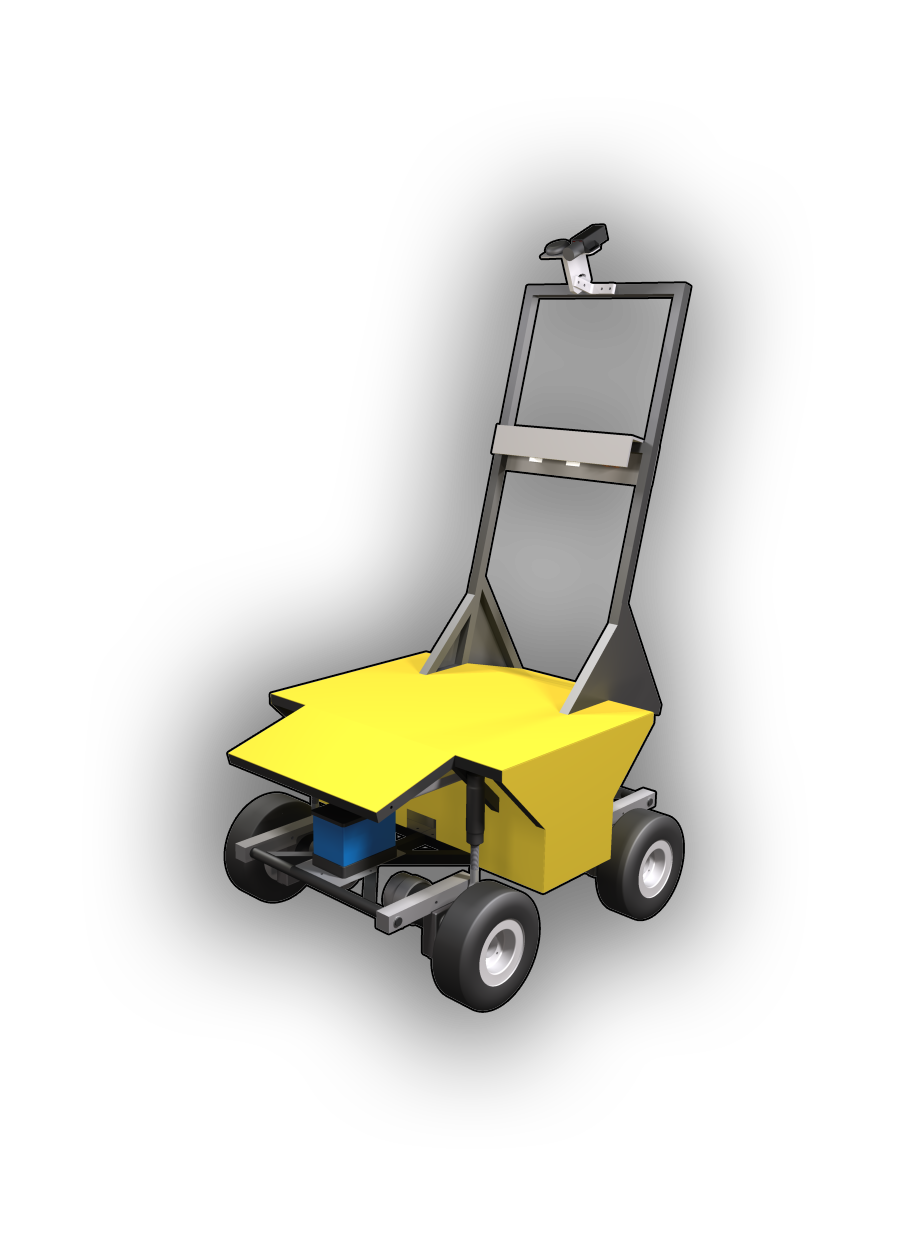
\includegraphics[width=4in]{./pics/RobotFrontCover.png}
\end{center}

%\newpage
%\begin{abstract}
abstract lorem ipsum
\end{abstract}


\newpage
%\section*{Table of Contents}
\setcounter{tocdepth}{2}
\tableofcontents

\newpage
%\section*{List of figures \& Tables}
\listoffigures
\listoftables

\newpage
\section{Introduction}

\subsection{RoboJackets}

%stuff about club and teams
RoboJackets is a robotics competition and outreach group that has been operating at the Georgia Institute of Technology since 1999. Overall the RoboJackets consist of four teams a FIRST outreach / mentorship, Middle Weight BattleBots, RoboCup Small Size and IGVC. In all members come from many of the engineering departments across campus (prominently Mechanical, Aerospace, Electrical, and Computer Science) thus providing a truly multidisciplinary robotics development experience. The RoboJackets IGVC Team initially started in 2004 has fielded a team every year except 2005. Additionally, we have attained a top ten finish in the autonomous course since 2007. 

\subsection{Team Members}

The 2012 team members are listed in Table \ref{TAB:RJTeam}.

\begin{table}[H]
\begin{center}
\caption{2012 RoboJackets / IGVC Team}
\begin{tabular}{| l | p{2.4in} | p{2in} |}
\hline
Name & Degree / Class & Role\\ \hline
Thomas Evans &		BS Mechanical Engineering / Junior& Mechanical design and build\\ \hline
William Evans &		BS Mechanical Engineering / Junior& Mechanical design and build\\ \hline
Paul Foster &		BS Biomedical Engineering / Senior& Software, Electronics\\ \hline
Joe Hickey &		BS Mechanical Engineering / Junior&	Mechanical Lead\\ \hline
Emanuel Jones &		BS Mechanical Engineering / Senior& Mechanical desing and build\\ \hline
Andrey Kurenkov &	BS Computer Science / Freshman & Software, Electronics\\ \hline
Michael Lelak &		BS Mechanical Engineering / Junior& Mechanical design and build\\ \hline
Kenneth Marino &	BS Computer Engineering / Sophomore&	Project Manager, Software, Electronics\\ \hline
Stefan Posey &		BS Aerospace Engineering / Senior &		Mechanical build\\ \hline
Haoxiang Yang &		BS Electrical Engineering / Sophomore & Software, electronics\\ \hline
Zhixun Wu &			BS Electrical Engineering / Sophomore &	Software, electronics\\ \hline 



\end{tabular}
\label{TAB:RJTeam}
\end{center}
\end{table}


%\newpage
%\section{Overall Design}




%\newpage
\section{Mechanical Design}

\subsection{Structure \& Vehicle Layout Overview}


\begin{figure}[H]
\begin{center}
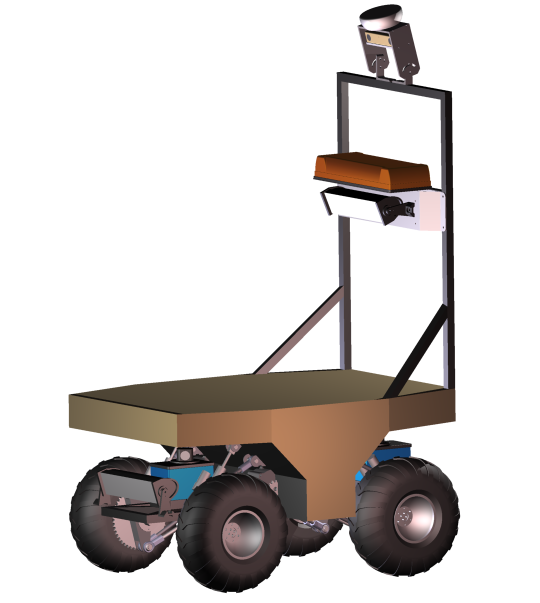
\includegraphics[width=3in]{./Pics/Misti_Vehicle.png}
\caption{Misti, the 2012-2013 Base}

\label{FIG:Misti}
\end{center}
\end{figure}

While the team did moderately well in the 2012 competition, certain areas of improvement were noted and emphasized in this year's design. Similar to the previous three years, the design revolved around a four-wheeled drive platform, with focus on reducing build complexity and increasing ease of vehicle maintenance (i.e. accessibility to components, proper wire routing, etc.) The team approached the 2013 design with the following goals:

\begin{enumerate}
\item Improve Vehicle Ride Dynamics
\item Increase Ground Clearance
\item Improve Human Interface for Debugging
\item Weatherproofing for Inclement Weather 
\item Enhance Night-Time Operability
\end{enumerate}

By following these goals, the team developed the current vehicle which boasts a vastly superior suspension system and drivetrain, as well as much improved component layout and accessibility.

\subsection{Vehicle Ride Dynamics}
\subsubsection{Drive System}
The vehicle, dubbed Misti, has a completely customized drivetrain designed to deliver high torque for operating on rough terrain.

The two central gearboxes, custom-made and milled from aluminum, are driven by 4.5 peak horsepower Ampflow A28-400 brushed DC motors. Gear reduction comes from a two-stage gear train inside the gearbox, as seen in Figures \ref{FIG:Gearbox} and \ref{FIG:Explode}, with the output sprocket driving a chain connected to a sprocket affixed to the wheel, producing a total reduction of 30 to 1. The skid-steer approach was maintained from the previous 3 competitions, but the fore and aft wheels are now mechanically linked together to ensure they maintain the same speed. This guarantees that under slippery conditions, the power is always transmitted to the ground through the wheel with the most traction. 

\begin{figure}[H]
\begin{minipage}[b]{0.5\linewidth}
\centering
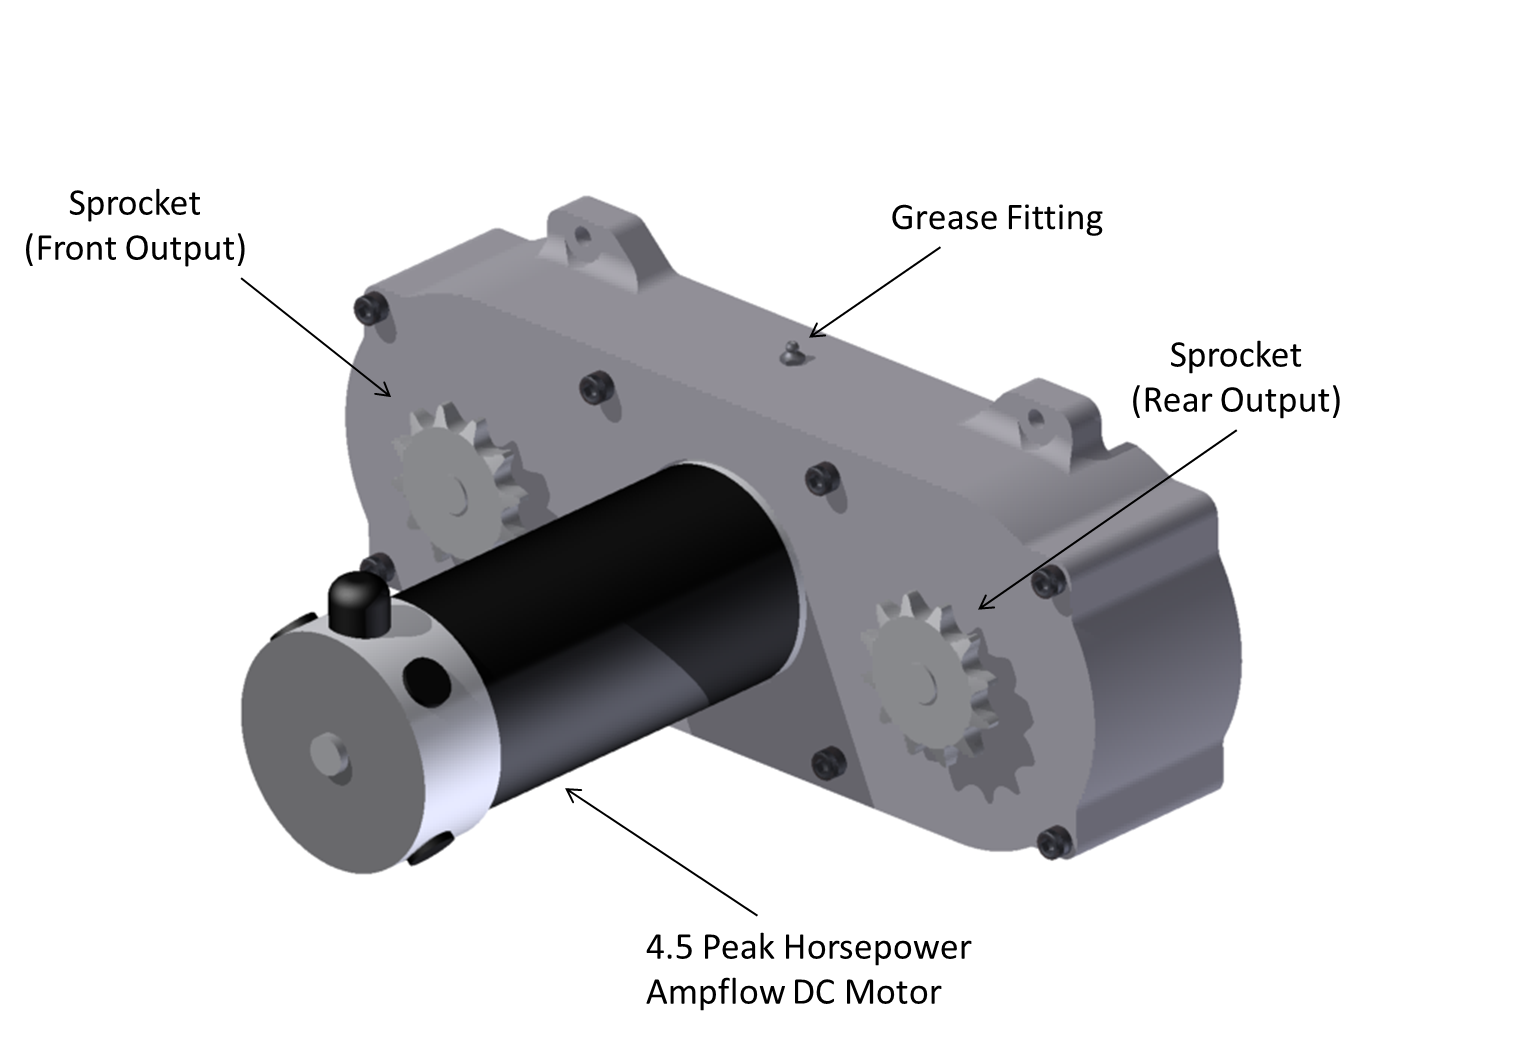
\includegraphics[width=3in]{./Pics/GearboxAssembled.png}
\caption{Custom Gearbox}
\label{FIG:Gearbox}
\end{minipage}
\hspace{0.1in}
\begin{minipage}[b]{0.5\linewidth}
\centering
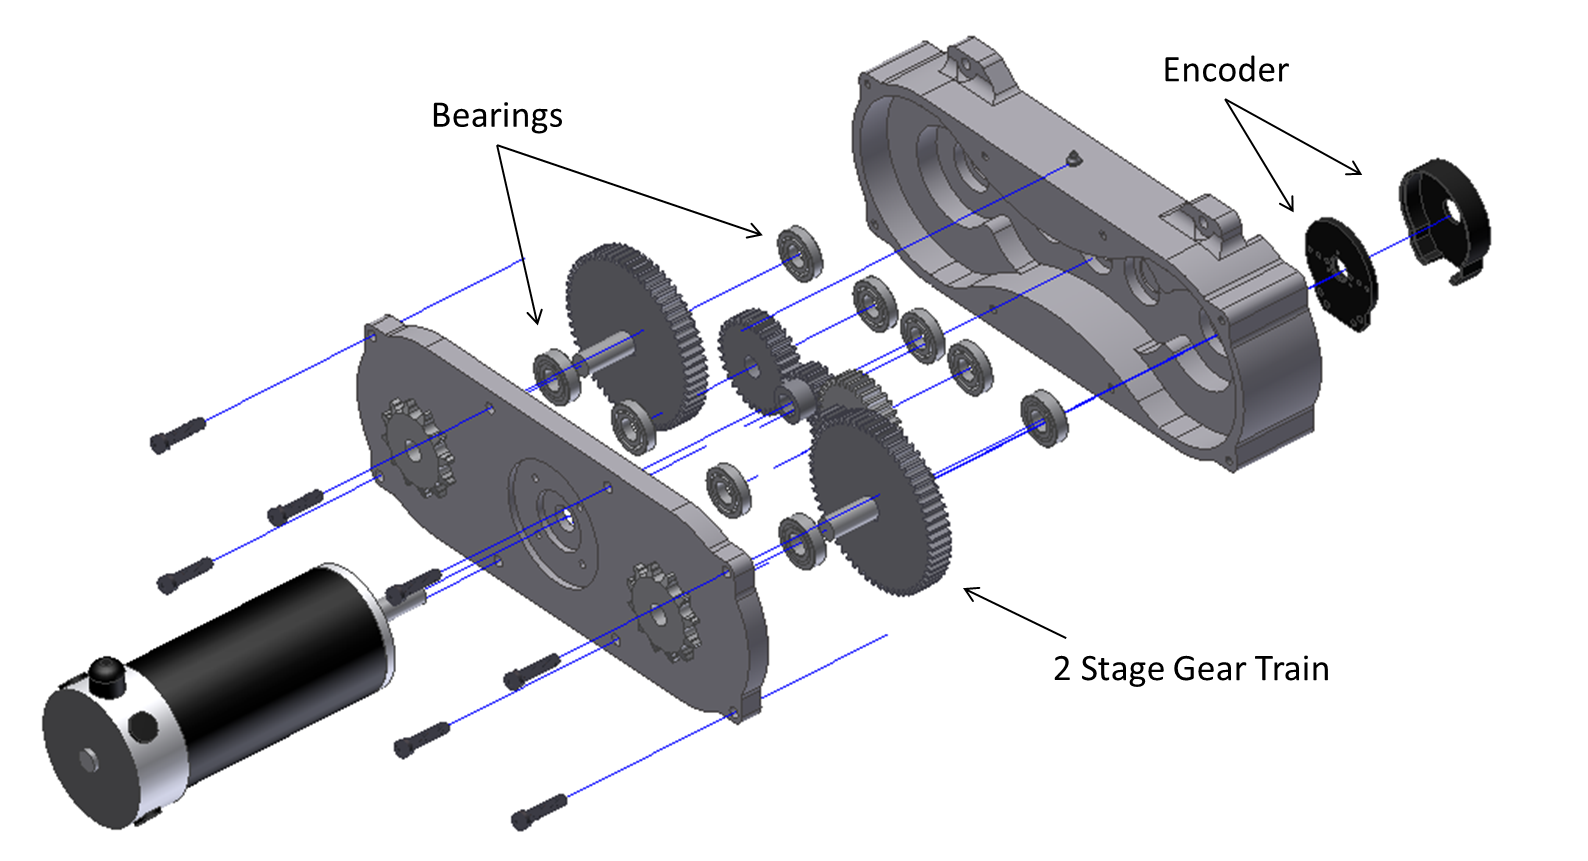
\includegraphics[width=3in]{./Pics/GearboxExploded.png}
\caption{Exploded View of Gearbox}
\label{FIG:Explode}
\end{minipage}
\end{figure}


\subsubsection{Suspension}
The suspension of the robot was greatly improved over the previous year’s design. Prior designs utilized a trailing/leading arm suspension system, connected away from the main body of the robot. This year, a four bar linkage mounted to the middle section of the robot was developed in order to reduce the cyclic loading on the frame as well as improve the damping characteristics  (see Figure \ref{FIG:Shock}). Fox DHX RC4 coilover dampers were a much welcomed improvement over previous homemade solutions. The suspension design allows for approximately 5 inches of travel for each wheel, lending the design much superior ride dynamics to ensure stability and dampened impacts while traversing rough terrain.
Misti was designed to handle even the roughest of conditions with nearly 8 inches of ground clearance. Using 145/70-6 pneumatic wheels, she can roll over most common obstacles with ease. The larger wheels will improve our ability to traverse small obstacles and climb ramps. While pneumatic tires do offer the potential to go flat, unlike our previous foam core tires, it was determined they would provide a superior ride dynamic and cushion small bumps, particularly at lower speeds.
\begin{figure}[H]
\begin{center}
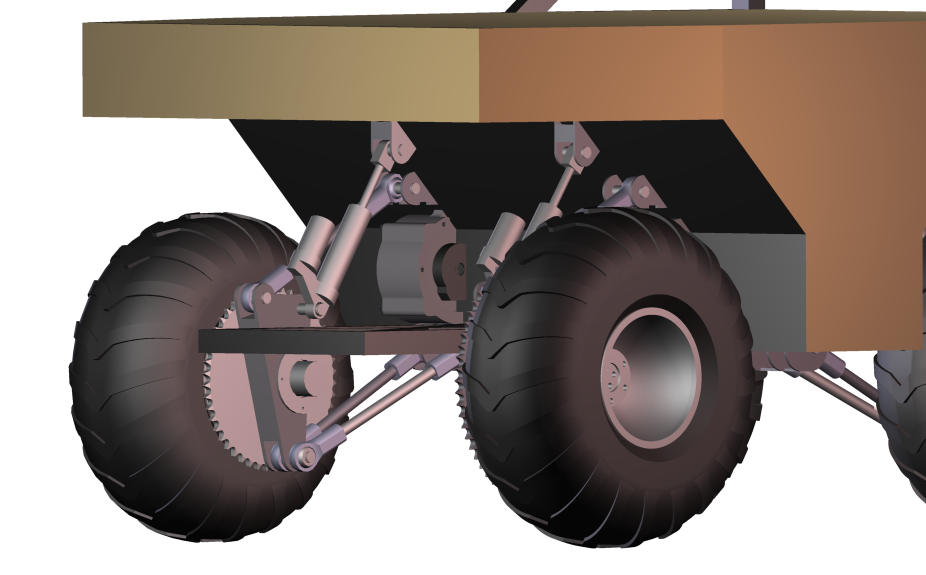
\includegraphics[width=3in]{./Pics/Suspension-Far.png}
\caption{Shock System}
\label{FIG:Shock}
\end{center}
\end{figure}



\subsection{Frame}
The frame is constructed out of 1/16" wall 1" sq. steel tube and aluminum panels. Much of the assembly was accomplished with MIG welding and the use of 1/4-20 fasteners. A model of the frame was made in Siemens NX and finite element analysis was conducted using the NASTRAN package. A stress analysis was performed using half inch tetrahedral elements to determine if the robot would be safe to pick up for maintenance and loading for events. The analysis assumed that the final assembly would have a weight of 500 pounds, overestimating the total weight to give a worst case scenario. When the force to lift the robot was applied to each end, the maximum stresses were found to be $2.33x10^4$ psi. This result is shown in Figure \ref{FIG:stress}.


\begin{figure}[H]
\begin{center}
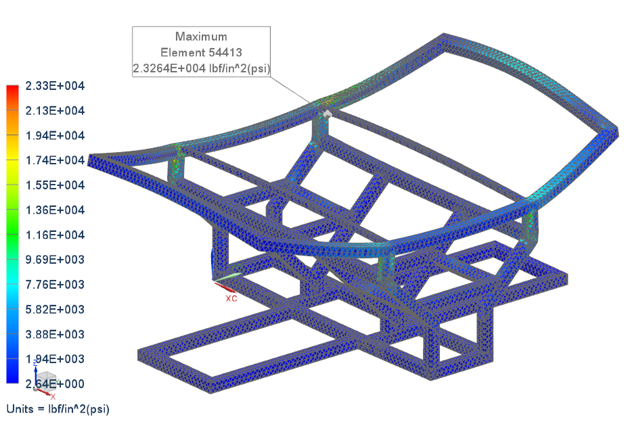
\includegraphics[width=3in]{./Pics/Stress.png}
\caption{Finite Element Streses}
\label{FIG:stress}
\end{center}
\end{figure}

Because this stress is lower than the yield stress of carbon steel of $5x10^5$ psi, a fatigue analysis was conducted to determine how it would behave after one million cycles. Figure \ref{FIG:cycles} shows the number of cycles to failure as predicted by the simulation.

\begin{figure}[H]
\begin{center}
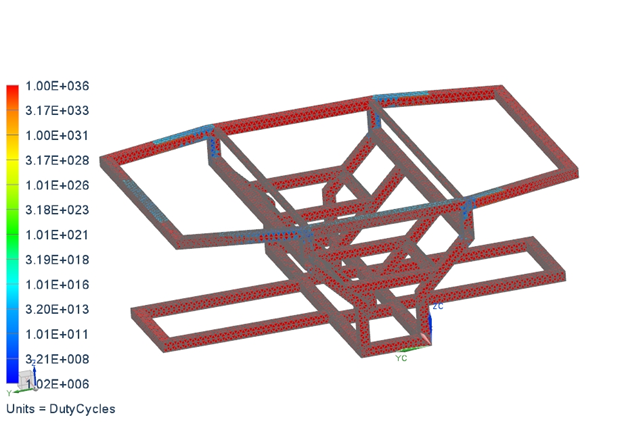
\includegraphics[width=3in]{./Pics/Cycles.png}
\caption{Cycles to Failure}
\label{FIG:cycles}
\end{center}
\end{figure}

The finite element analysis predicted that the frame would last at least 1 million cycles in the worst case scenarios under this loading condition. Also, it predicted a safety factor of 2.89 at the corner where the stresses were highest. Since the model was assumed to be heavier than the true weight and the joints are also reinforced with steel plates, this safety factor is sufficient.


\subsection{Mast}
A vertical mast on the aft of the robot supports the GPS, IMU, and stereoscopic camera, as well as a button panel for operating the lights, emergency stop and go buttons (Figure \ref{FIG:mast}).
\begin{figure}[H]
\begin{center}
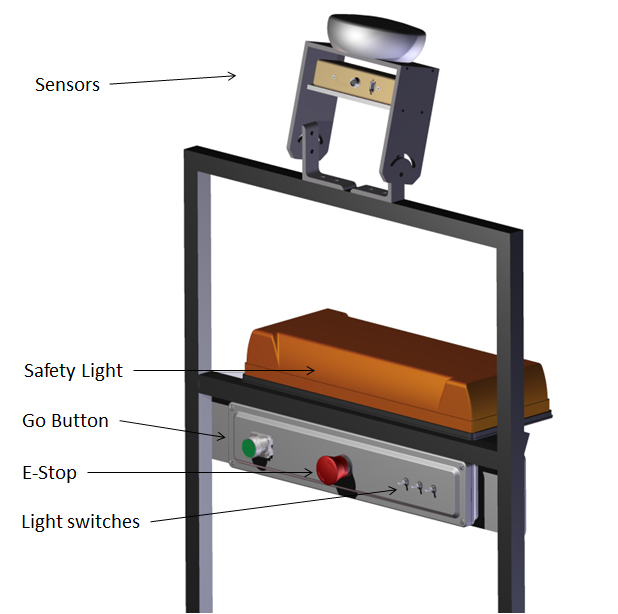
\includegraphics[width=3in]{./Pics/Mast.png}
\caption{Mast}
\label{FIG:mast}
\end{center}
\end{figure}

The mast, which stands 67 inches tall, was designed to give the camera sufficient field of view, while also being just low enough to easily fit inside the RoboJackets’ transportation trailer for ease of travel. The button panel, and particularly the E-stop, resides at forehead height (Figure \ref{FIG:forehead}) with respect to the stance of the user while operating/debugging code onboard computer, a design feature intended to prevent injury in case the robot malfunctions and moves backwards. Components that are exposed to the elements have been weatherproofed by using wash-down enclosures. This provides added robustness, allowing the team to test in inclement weather without worry.
\begin{figure}[H]
\begin{center}
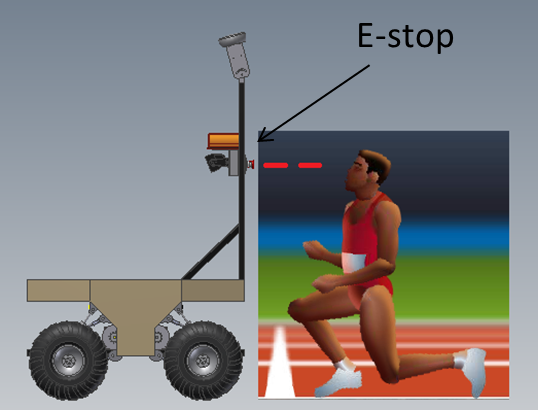
\includegraphics[width=3in]{./Pics/QWOP.png}
\caption{E-Stop at Forehead Height}
\label{FIG:forehead}
\end{center}
\end{figure}

The sensor loadout (Figure \ref{FIG:sensors}) includes a stereoscopic camera, GPS unit, and inertial measurement unit (IMU) on the mast, as well as a LIDAR residing on the bottom of the robot frame and an encoder in each gearbox.

\begin{figure}[H]
\begin{center}
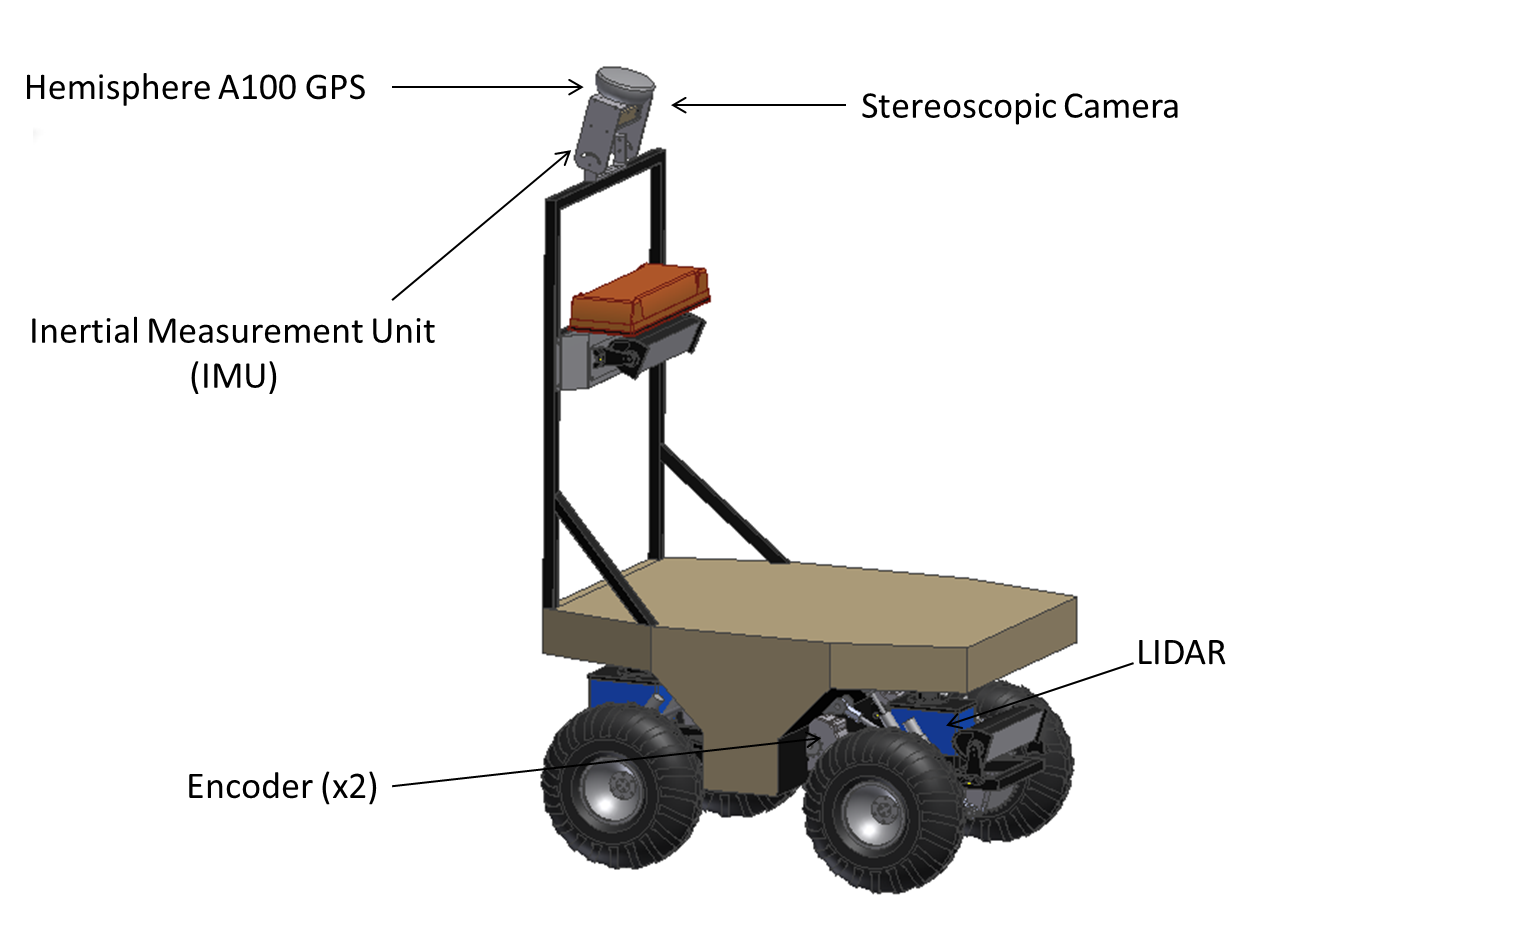
\includegraphics[width=4in]{./Pics/Sensors.png}
\caption{Sensor Loadout}
\label{FIG:sensors}
\end{center}
\end{figure}

To boost safety and night-time/dusk operability, the team installed a large safety light, as well as two large headlights (Figure \ref{FIG:lights}) to light the field both close and far from the vehicle.

\begin{figure}[H]
\begin{center}
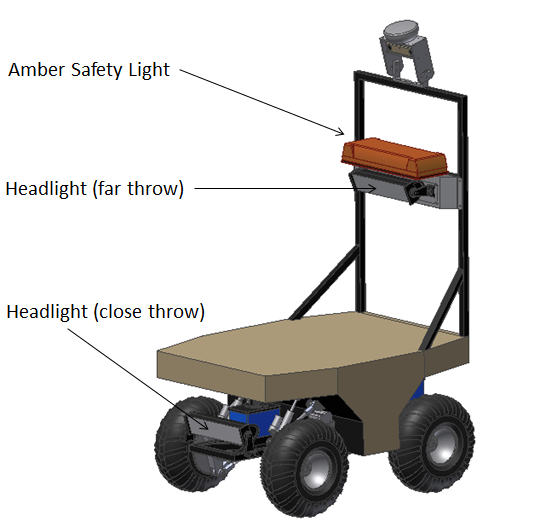
\includegraphics[width=3in]{./Pics/Lighting.png}
\caption{Lights}
\label{FIG:lights}
\end{center}
\end{figure}


\subsection{LIDAR}
% Mention LIDAR FOV protection from rain, accessibility. How it comes off with 3 bolts, etc.
The modified SICK NAV 200 LIDAR is mounted in the front of the vehicle and has an unobstructed sweep of roughly 150 degrees. The LIDAR is protected above from rain by an overhang which also serves as a compartment for the electrical power system. The unit is attached to the base through an intermediate aluminum plate. This allows it to be removed from the vehicle with only loosening three 1/4-20 bolts which are the standard fastener for our platform.


%\newpage
\section{Electronics Design}

The electronics for Roxi can be broken into three major catagories: Senors, Power, and computers.

\subsection{Sensors}

Roxi uses vision and LIDAR as its primary sensors used for the navigation challenge and also has GPS and wheel encoders to allow for waypoint navigation.

\subsubsection{Vision}

The vision system consists of a AVT Guppy F-036C camera connected via an IEEE 1394a link to the main computer. This camera is capable of 752 x 480 resolution at 64 fps. This camera is polled at approximately 10 Hz to send a new frame to the vision algorithm.  The camera is placed at the top of the mast, facing forwards and down to allow the lines and obstacle in front of the robot to be sensed.

\subsubsection{Wheel Encoder}

Each wheel is connected to a quadrature wheel encoder, allowing wheel rate to be measured. This allows the velocity of the robot to be measured. The encoder is a US Digital E3-200-375-I-H-M-B, with 200 counts per revolution and an index channel. This allows for wheel rates up to XX speed to be sensed. The quadrature lines drive interrupts on a microcontroller, which then feeds the state of the lines to a state machine which increments or decrements a wheel counter. Wheel angular velocity is measured by differencing the number of counts over a 5 ms period, allowing a bandwidth of XX Hz and XX m / s. The microcontrollers are capable of sending both rate and count information to the laptop, allowing for speed control and odometry operations.

\subsubsection{LIDAR}

Two front and rear mounted Sick NAV300 LIDAR are used as object and ramp detectors. The LIDAR have a $270^{\circ}$ FOV and a 10 meter range. The front facing LIDAR is used as an object finder, while the back facing LIDAR is used as a safety feature allowing the robot to sense if an object / person is moved behind it after the robot has moved through an area.

\subsubsection{GPS}

A GPS is used

\subsection{Power}

\subsubsection{Main Power}

Main power for the robot comes from two sealed lead acid gell-cell batteries. These batteries are connected in series to produce a nominal 24 VDC supply for the motors and other systems. This provides approximatly XX $W \cdot hr$ of energy, XX hours of runtime of the motors, and XX hours of runtime of the electronics and motors.

The batteries are connected to a power distribution board, which allows the connection to each motor to be fused with XX Amps, allowing power to be cut in the event of a motor stall to prevent damage to the H-bridge. Power is also provided to several DC-DC boost converters, which output 5 VDC, 9 VDC, and 19.5 VDC for other electronics on the robot.

\subsubsection{H Bridge}

Each motor is connected to an OSMC H-bridge. This board is used to allow a low power signal from the microcontrollers to generate a high power PWM input to the motors. Each OSMC is capible of switching up to 50 VDC at 160A cont / 300A peak, allowing significant margin above our standard operating power of around 24 VDC / 20 A.

\subsubsection{Component Power}

Other systems are provided power through the use of DC-DC converters to produce voltages at 5 V, 9 V, and 19.5 V. This allows for the usb tethered microcontrollers, the firewire camera, and the main computer to be powered off of the main lead acid batteries. This greatly simplifies charging the robot, as only one battery system needs to be maintained.

\subsection{Computers}

\subsubsection{Main Computer}

Nearly all computation is performed on a single laptop containing a quadcore Intel Core i7 cpu, cuda enabled NVIDIA 285M gpu, and 6 GB of RAM. This computer is responsible for all vision, lidar, and GPS data processing and all path planning and control algoritms. It also forms the core of the sensor interconects, providing the firewire and USB bus the camera, GPS, and microcontrollers use.

\subsubsection{MCU}

Microcontrollers are used on Roxi as data aquisition boards to collect data from the wheel encoders, and as motor control boards to generate PWM signals to drive the H-bridges. There are 6 ATmega328p based Arduino Duemilanove boards on the robot, 4 interfacing with the wheel encoders, and 2 to drive the motors.


%\newpage
\section{Software Design}

\subsection{Architecture}

\subsection{Algorithms}

\subsubsection{vision}

The robot uses vision as the primary method of detecting obstacles and lines. The vision algorithm has been developed and modified over several years of competition and is considered reasonably robust. After passing the input video through several different algorithms, a short-term map of the world is created, which the robot is driven off of.

The input video, above-left, is first passed through an inverse perspective transform, as seen above-right. This transform makes both near and far off objects a normalized size, and makes the image appear to be taken from directly overhead. This flattened image assumes the course is a plane, which does cause distortion of the barrels, but this is accounted for in the mapping algorithm. The transformed image is much easier to process into a map than a normal, perspective image would be.

The images is then color segmented and thresholded based on the color that is centered directly in front of the robot, as seen above. Safe colors are marked white, the rest are black. The color is averaged in time between frames to allow for some variation in color, for example, if there is dead pach in the grass. This allows the robot to operate on many different surfaces with the same software. For testing we have operated on asphalt parking lots, navigating between the lines marking parking spaces.

After converting the transformed image to grayscale, feature tracking is preformed between subsequent frames. The tracked features are denoted by the black lines in the above grayscale image. The algorithm looks for features that have been translated and rotated between frames. This allows us to build a set of likely homographic transform between the images, which can be backed out into likely robot motion between frames. The possible homographic transforms often include several incorrectly matched points, so RANSAC, a nonlinear filter good at outlier handling, is used to reject the outliers and select the best transform.

Using motion data, camera frames are drawn into the world map, shown to the right above. The map is a grayscale image, representing a probabilty function of traversablility, where black (0) represents non-traversable, gray (127) represents unknown areas and white(0) represents traversable ares. The map is built up as the robot moves, and slowly decays back to gray to prevent loop closure errors from building up. This map allows the robot to “remember” that it just passed an obstacle and needs to not turn sharply in order to avoid a collision. The robot is driven from the map, by a path planning algorithm.

\subsubsection{Path Planning}


%\newpage
\section{Performance}

The main goals of the new base was modifying the suspension to allow for higher operating speeds. The old mechanical base, Jeanni, did not have enough travel on its shocks to allow for very high speed operation. The increased travel will also make going onto and off the ramp less jarring. The robot is capable of XX hours of runtime running all systems.

As we are using a legacy vision and control algorithm that has been capable of avoiding obsticals and navigating switchbacks on a mechanical base of almost the same form factor, we are confident that the software will continue to perform as well as it has in the past.

Using the camera, objects come into view at a distance of 2 m. The LIDAR allows objects to be sensed reliably at up to 5 m. The robot will typically begin to take action at a distance of 1 m - 2 m.

\newpage
\section{Cost}

The bill of materials and estimated cost for Roxi is included in Table \ref{TAB:Cost}. The robot cost about \$6500, with some materials bought used and/or reused from previous years.

\begin{table}[H]
\begin{center}
\caption{Roxi BOM}
\begin{tabular}{| l | c |}
\hline

Steel	&	400\\	\hline
Aluminum	&	200\\	\hline
Misc Mechanical	&	300\\	\hline
Dampers	&	200\\	\hline
Springs	&	20\\	\hline
4x Motors / Wheels	&	1400\\	\hline
4x OSMC Motor Controller	&	680\\	\hline
2x LIDAR	&	100\\	\hline
Camera	&	580\\	\hline
Camera lens	&	140\\	\hline
Motor Interface board	&	30\\	\hline
Misc Cables	&	50\\	\hline
4x Wheel Encoder	&	355\\	\hline
6x Arduino	&	185\\	\hline
2x Motor Interface Shield	&	40\\	\hline
Estop	&	80\\	\hline
Current Sensors	&	20\\	\hline
Laptop	&	1300\\	\hline
Firewire express card	&	40\\	\hline
Polycarbonate Sheets	&	130\\	\hline
Power Inverter	&	50\\	\hline
DC/DC Converter	&	50\\	\hline
Paint	&	30\\	\hline
2x GPS	&	100\\	\hline
Total	&	\$6480\\	
\hline


\end{tabular}
\label{TAB:Cost}
\end{center}
\end{table}

This project was made possible through the support of Northrup Grumman, Caterpillar, General Motors, Lockheed Martin, National Instruments, United Technologies Corp., SGA, the George W. Woodruff School of Mechanical Engineering, the College of Computing, and the  Robotics and Intelligent Machines research center.

%\newpage
%\clearpage
\phantomsection
\addcontentsline{toc}{section}{References}
\nocite{*}
\bibliographystyle{plain}
\bibliography{igvc_paper_2011}


\end{document}
